\begin{figure}[htbp]
    \centering
    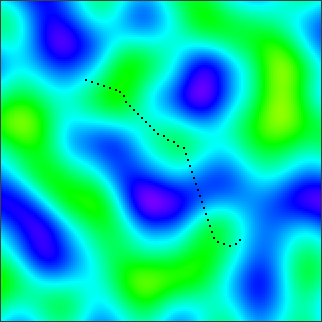
\includegraphics[scale=0.5]{a-star0}
    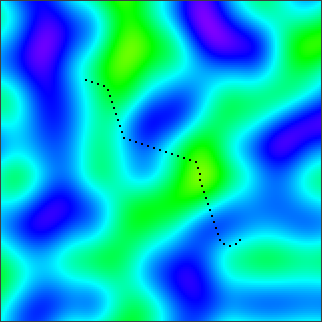
\includegraphics[scale=0.5]{a-star1}
    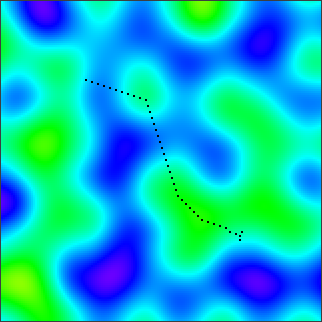
\includegraphics[scale=0.5]{a-star2}
    \caption{
        Three runs of the Nav. Green areas are relatively flat. Blue areas are steeper slopes; traversal through these
        areas is to be kept to a minimum.
    }\label{fig:nav-tests}
\end{figure}

\begin{figure}[htbp]
    \centering
    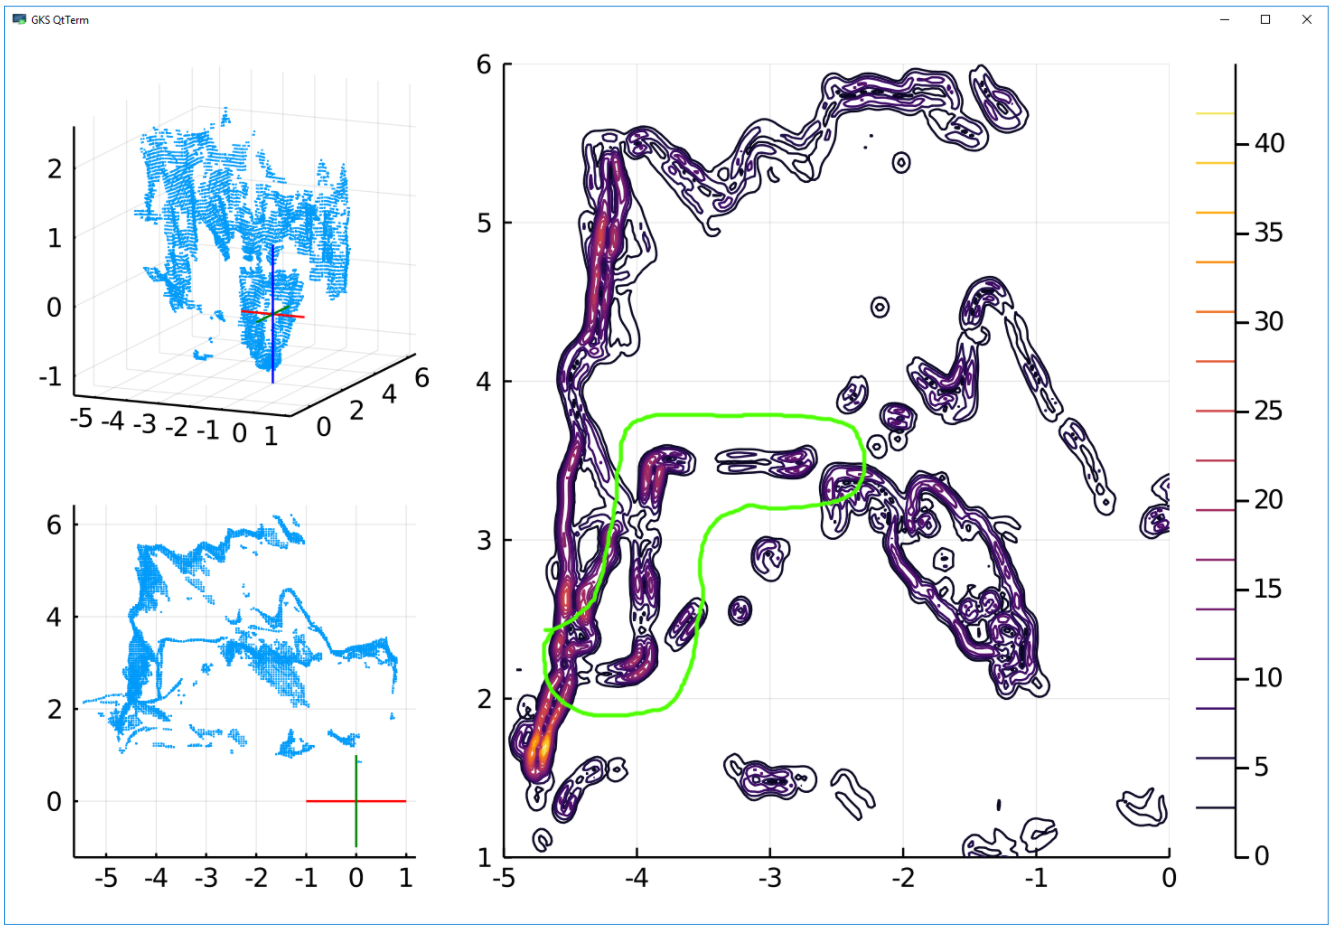
\includegraphics[scale=0.45]{mesh-to-grid-old}
    \caption{
        Visualization of the mesh to gradient grid conversion. The structure circled in green is an overhang with vertical walls that could be passed under, but this mapping would suggest otherwise.\linebreak
        Top-left: Mesh vertices viewed from an oblique angle\linebreak
        Bottom-left: Mesh vertices viewed from above\linebreak
        Right: Contour plot of the gradient magnitude
    }
\end{figure}

\begin{figure}[htbp]
    \centering
    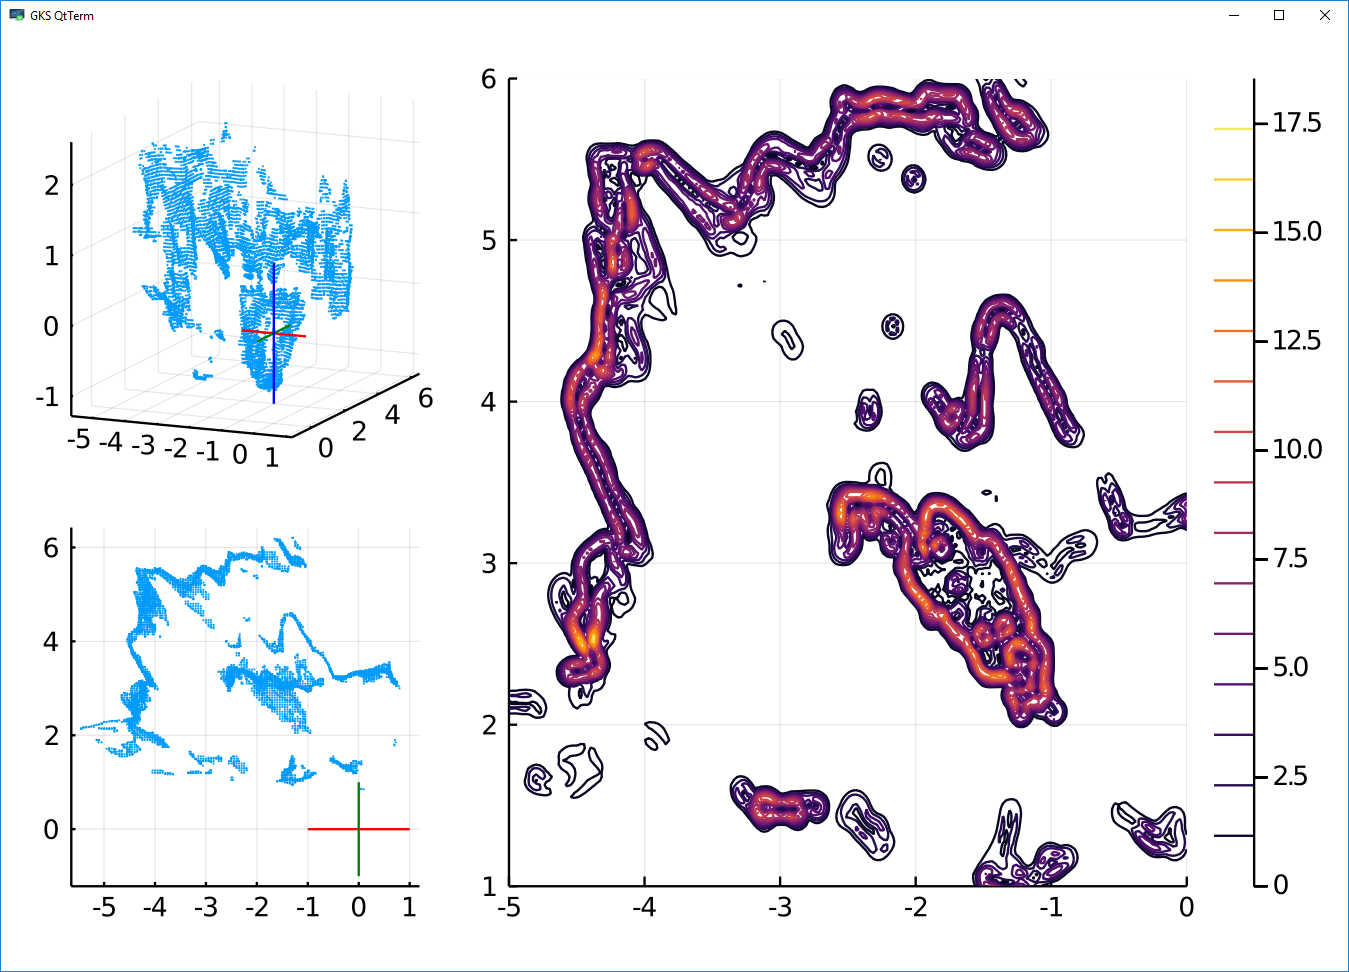
\includegraphics[scale=0.45]{mesh-to-grid}
    \caption{Improved mesh-to-grid. The overhang is no longer interpreted as a wall.}
\end{figure}
